\documentclass{article}
\usepackage{amsmath,amssymb,amsthm,kotex,paralist,mathrsfs}
\usepackage[labelsep=space]{caption}
\newcounter{num}[section]
\newcommand{\defi}[1]
{\bigskip\noindent\refstepcounter{num}\textbf{정의 \arabic{section}. \arabic{num}) #1}\par}
\newcommand{\theo}[1]
{\bigskip\noindent\refstepcounter{num}\textbf{정리 \arabic{section}. \arabic{num}) #1}\par}
\newcommand{\axio}[1]

\renewcommand{\figurename}{그림}
\renewcommand{\proofname}{증명}

\begin{document}

\title{현빈 : 07 삼각함수}
\author{}
\date{\today}
\maketitle

\section{삼각비(중학교 3학년 2학기 과정)}

\defi{삼각비}
\(\angle C=90^\circ\)인  직각삼각형 \(\triangle ABC\)에서 \(A\)의 대변을 \(a\), \(B\)의 대변을 \(b\), \(C\)의 대변을 \(c\)라고 할 때, 다음과 같이 삼각비를 정의한다.[그림 1]
\begin{gather*}
\sin\angle A=\frac ac\\
\cos\angle A=\frac bc\\
\tan\angle A=\frac ab
\end{gather*}
\begin{figure}[h]
\center
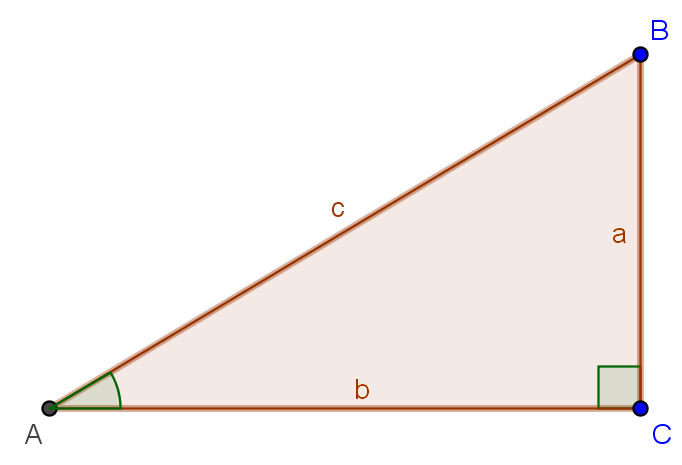
\includegraphics[width=0.5\textwidth]{trigonometric_ratios}
\caption{}
\end{figure}

이때 삼각비의 값은 주어진 각도에만 의존한다.
즉, 서로 다른 두 삼각형이라도 각도가 같으면 삼각비의 값은 같다.[그림 2]
\begin{figure}[h]
\center
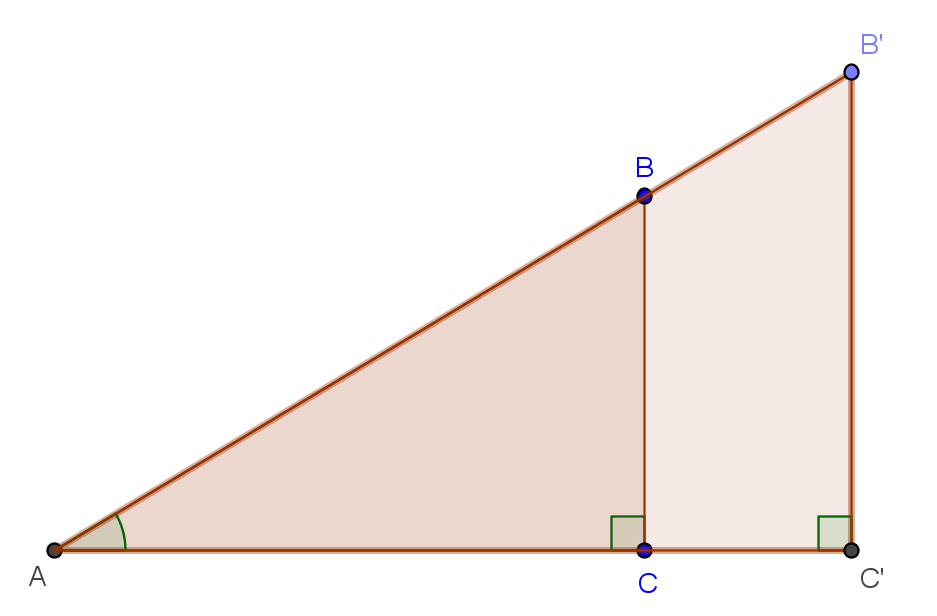
\includegraphics[width=0.5\textwidth]{trigonometric_ratios2}
\caption{}
\end{figure}

\theo{삼각비의 성질}
그림 3과 같이 사분면에서 반지름이 1인 사분원을 그리고 사분원 위의 한 점을 \(B\)라고 하자.
또 \(B\)에서 \(x\)축, \(y\)축에 내린 수선을 각각 \(D\), \(C\)라고 하자.
그리고 \(x\)축과 \(OB\)가 이루는 예각을 \(\theta\)라고 하면 다음이 성립한다.

(1)
\(\sin\theta=\overline{OC}\)이고 \(\cos\theta=\overline{OD}\)이다.

(2)
\(\sin^2\theta+\cos^2\theta=1\)이다.

(3)
\(0\le\sin\theta\le1\)이고 \(0\le\cos\theta\le1\)이다.

(4)
\(\tan\theta=\frac{\sin\theta}{\cos\theta}\)이다.
\begin{figure}[h]
\center
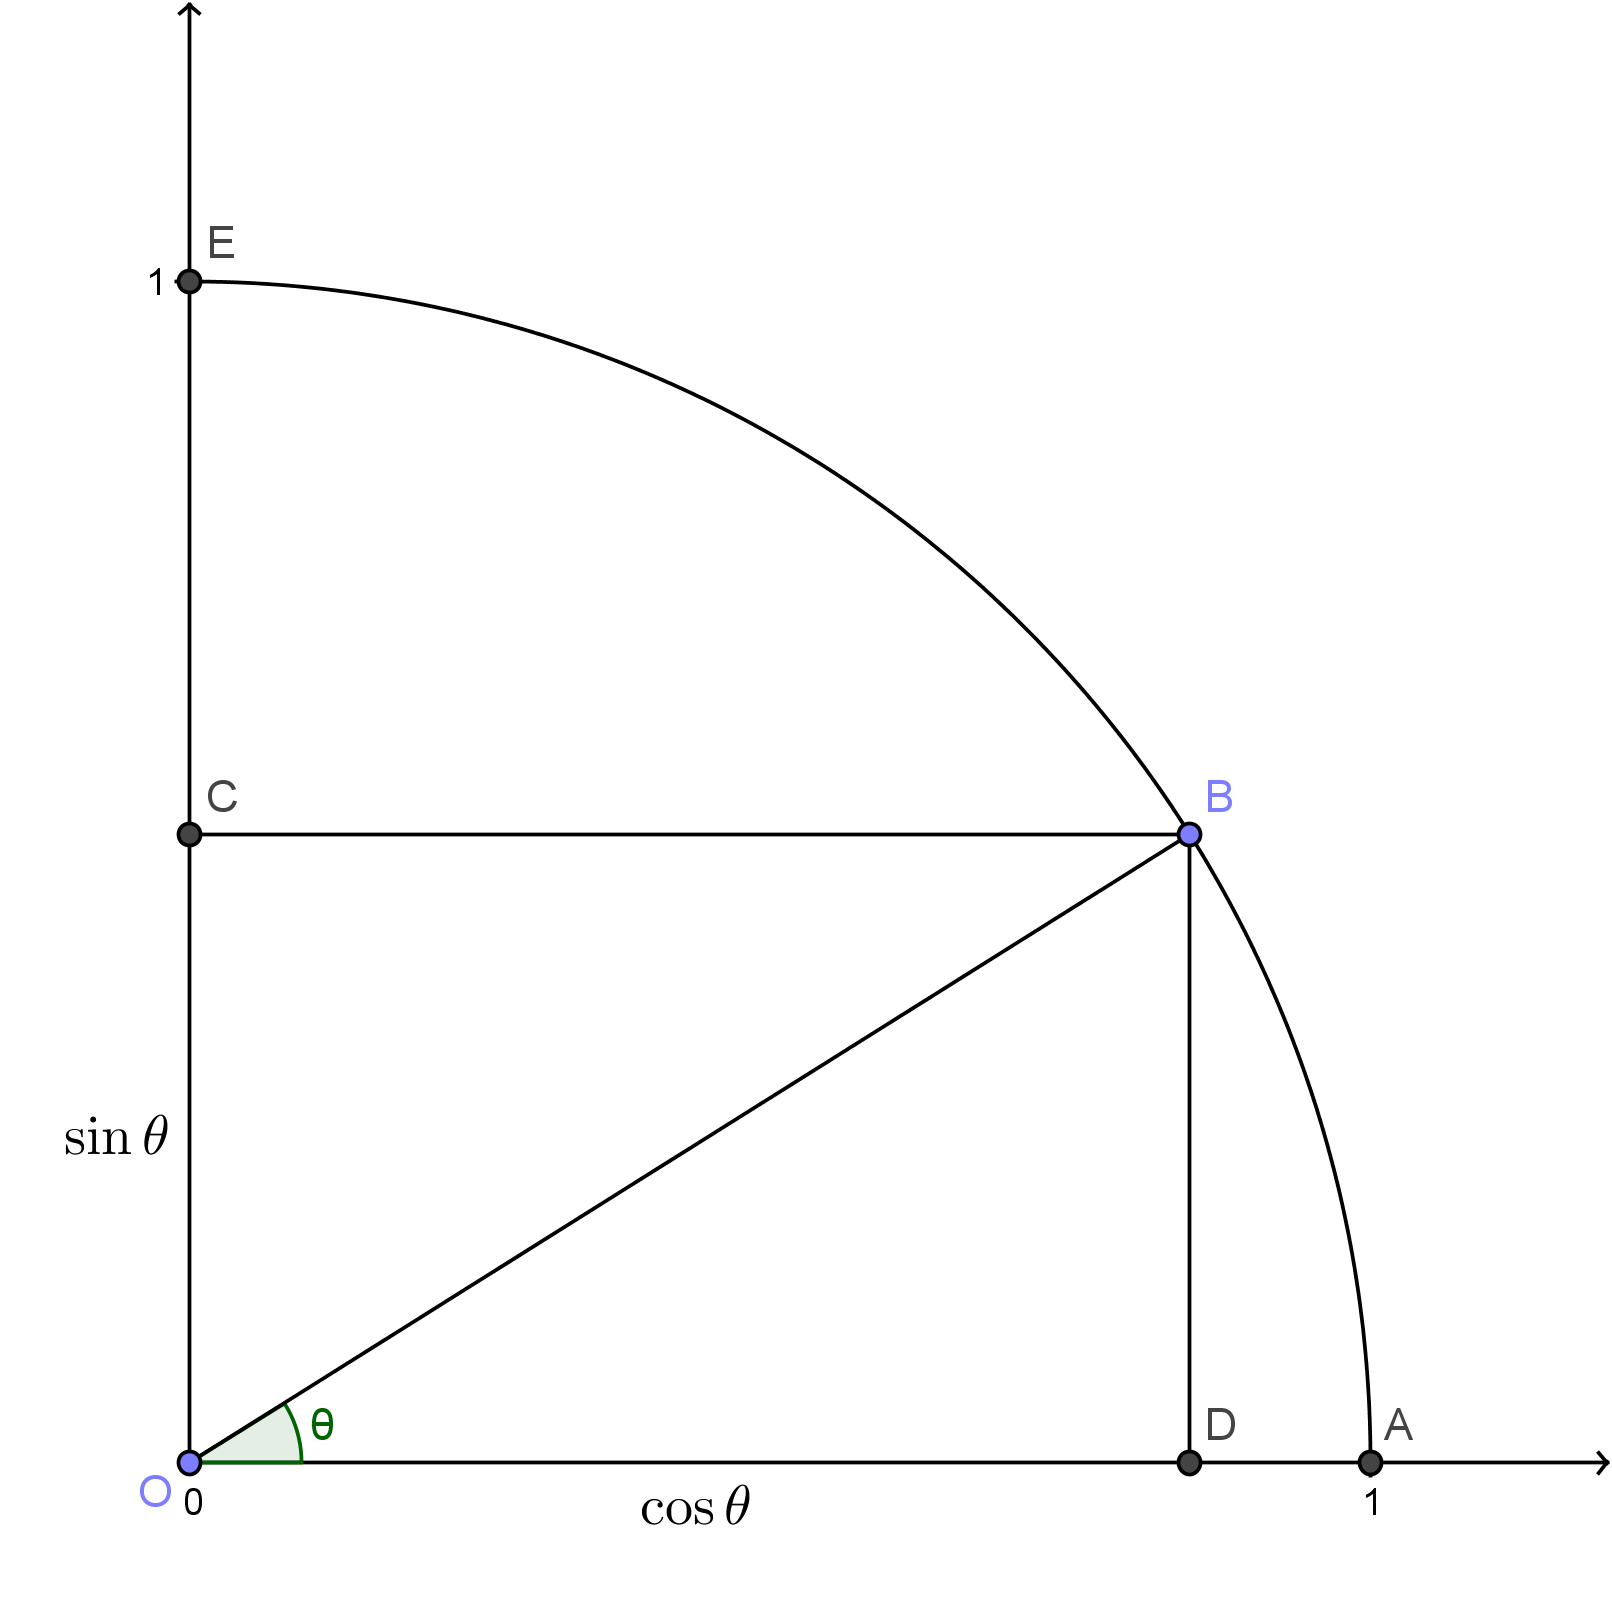
\includegraphics[width=0.5\textwidth]{trigonometric_ratios3}
\caption{}
\end{figure}

\section{삼각함수(고등학교 2학년 과정)}

\theo{원의 방정식}
좌표평면 상에 반지름의 길이가 \(r\)이고 중심이 원점인 원의 방정식은
\[x^2+y^2=r^2\]
이다.[그림 4]

\begin{figure}[h]
\center
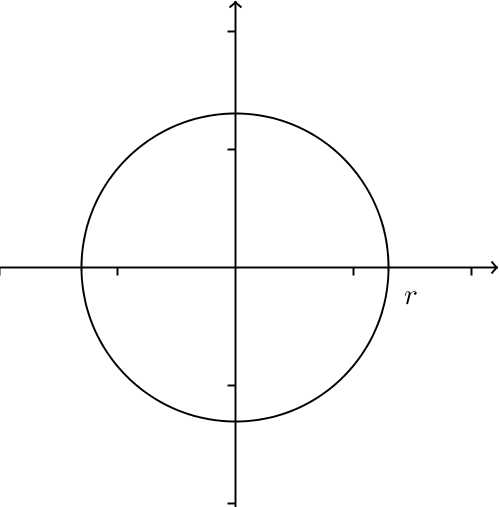
\includegraphics[width=0.5\textwidth]{circle}
\caption{}
\end{figure}

\begin{proof}
원이란, 한 점으로부터 일정한 거리(=반지름)에 있는 점들의 집합이다.
따라서 주어진 원 위의 임의의 점을 \(P(x,y)\)라고 하면, 이 점은
\[\overline{OP}=r\]
을 만족시켜야 한다(\(O\)는 원점).
\[\overline{OP}=\sqrt{x^2+y^2}\]
이므로 양변을 제곱하면
\[x^2+y^2=r^2\]
이 얻어진다.
\end{proof}

\defi{삼각함수}
좌표평면 상에 단위원(반지름의 길이가 1인 원)
\[
x^2+y^2=1
\]
을 생각하자.
\(A(1,0)\)로부터 원을 따라 시계반대방향으로 \(\theta\)만큼 이동시킨 점을 \(B\)라고 할 때
\(\sin\theta\)를 \(B\)의 \(y\)좌표, \(\cos\theta\)를 \(B\)의 \(x\)좌표로 정의한다.
\(\tan\theta\)는 \(\tan\theta=\frac{\sin\theta}{\cos\theta}\)로 정의한다.

따라서 그림 5에서처럼, \(B\)의 좌표는 \((\cos\theta,\sin\theta)\)이고, \(\tan\theta\)는 \(\overline{OB}\)의 기울기이다.
\begin{figure}[h]
\center
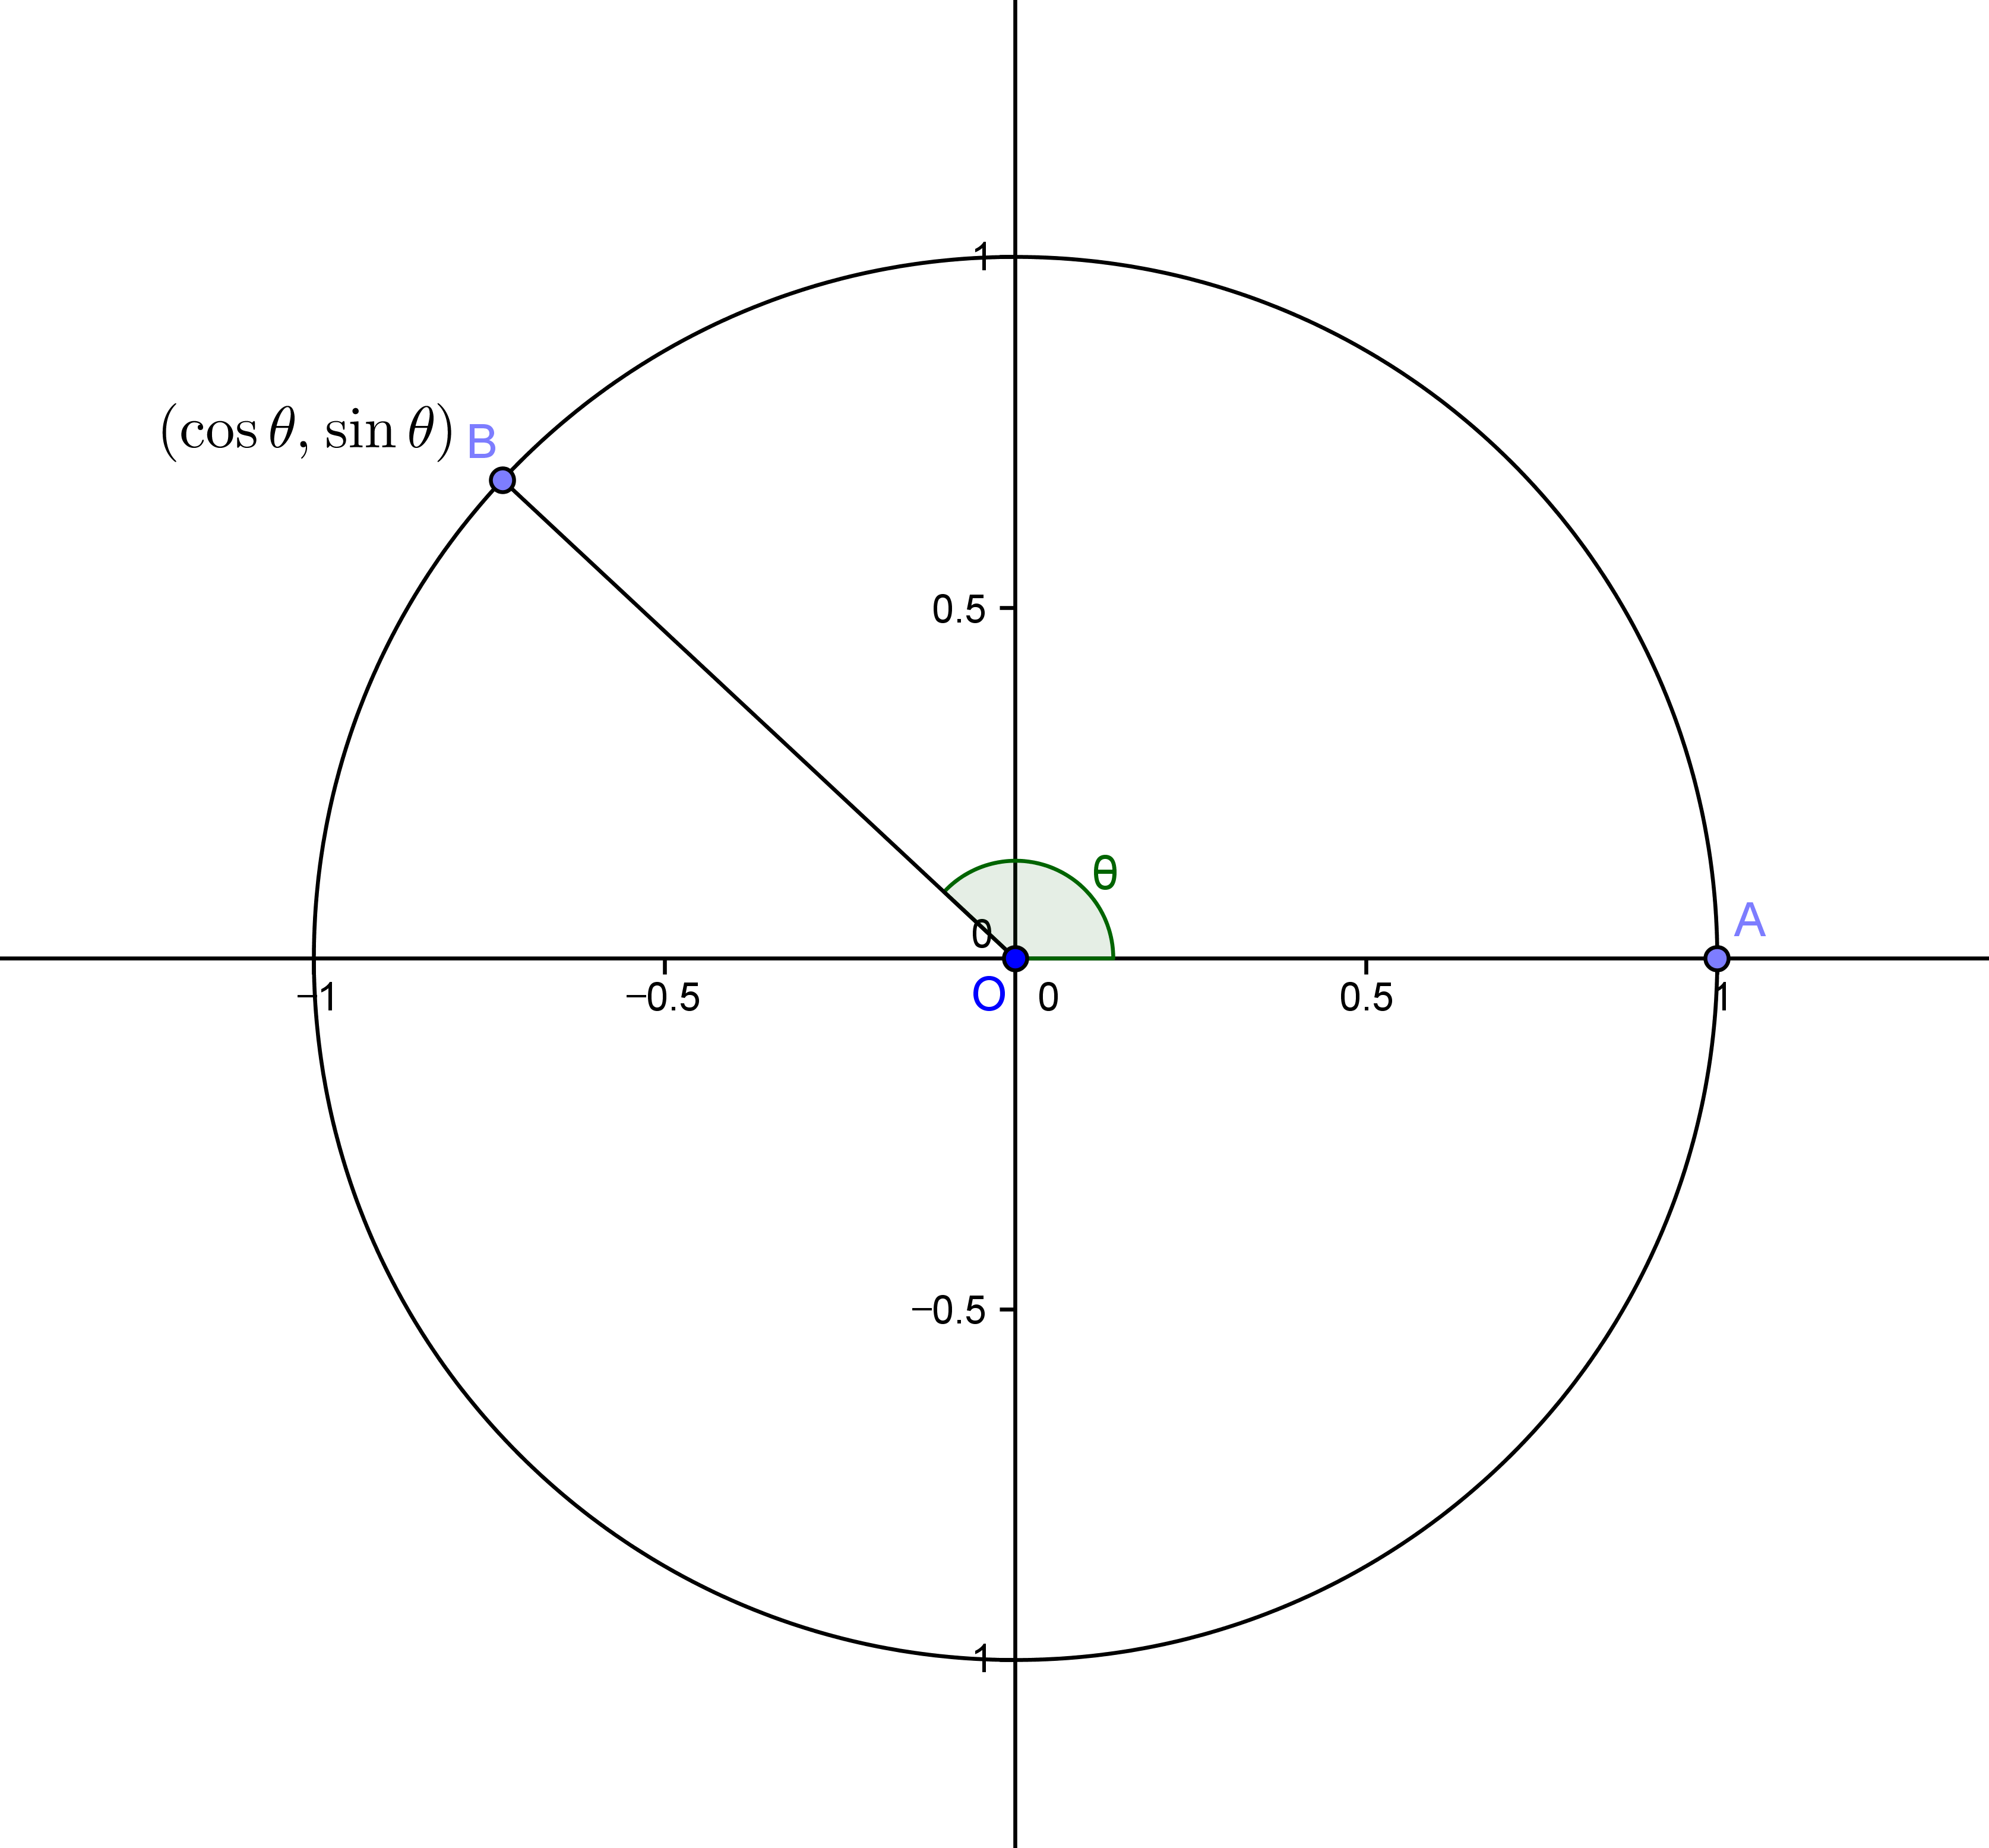
\includegraphics[width=\textwidth]{trigonometric_functions}
\caption{}
\end{figure}

이전 정의에서는 \(0^\circ\)에서 \(90^\circ\)까지의 사인, 코사인, 탄젠트값만을 정의했던 것과는 달리, 이번에는 모든 실수 각도에 대한 사인, 코사인 탄젠트값을 정의할 수 있었다.
또한 이 새로운 정의는 이전의 정의와  \(0^\circ\)에서 \(90^\circ\)까지의 범위에서 일치한다.

따라서 \(\sin\), \(\cos\), \(\tan\) 각각을 하나의 함수로서(정의역 = 실수전체) 간주할 수 있다.

\theo{삼각함수의 성질}
(1)
삼각함수는 \(360^\circ\)을 주기로 하는 주기함수이다.
즉 자연수 \(n\)에 대해
\begin{gather*}
\sin(\theta+360^\circ n)=\sin\theta\\
\cos(\theta+360^\circ n)=\cos\theta\\
\tan(\theta+360^\circ n)=\tan\theta
\end{gather*}
이다.

(2)
\(\sin^2\theta+\cos^2\theta=1\)이다.

(3)
\(-1\le\sin\theta\le1\)이고 \(-1\le\cos\theta\le1\)이다.
\end{document}